\documentclass[12pt]{article} % use larger type; default would be 10pt

\usepackage{pgfplots}
\usetikzlibrary{calc}
\usetikzlibrary{arrows}
\usetikzlibrary{patterns}
\usetikzlibrary{calc,intersections,through,backgrounds}
\usetikzlibrary{decorations.pathreplacing}
        \usepackage{xcolor} 
        \newcommand\degree[0]{^{\circ}}
        \newcommand\abs[1]{\left|#1\right|}
\usepackage{amsmath}
        \newcommand{\alert}[1]{\boldsymbol{\color{magenta}{#1}}}
        \newcommand{\blert}[1]{\boldsymbol{\color{blue}{#1}}}

\title{Play with TikZ}
\author{Just Us}
%\date{} % Activate to display a given date or no date (if empty),
         % otherwise the current date is printed 

\begin{document}
\maketitle

\section{Chap 9 Section 4}





hp-9-4-29 equilateral triangle

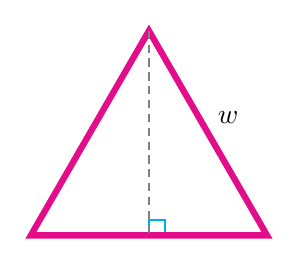
\begin{tikzpicture} 
\coordinate (A) at (0,0);
\coordinate (B) at (3,0);
\coordinate (C) at (60:3);
\coordinate (F) at (3/2,0);
\draw[cyan, thick] (F) rectangle ++(.2,.2);
\draw[magenta!95!black,  line width=.8mm] (A)--(B)--(C)--cycle;
\draw[gray, thick, densely dashed] (C)--(F);
\node [above right] at ($ (B)+(120:1.5)$) {$w$};
\end{tikzpicture}
\newline

\section{Chap 9 Section 5}



hp-9-5-6 square root graph


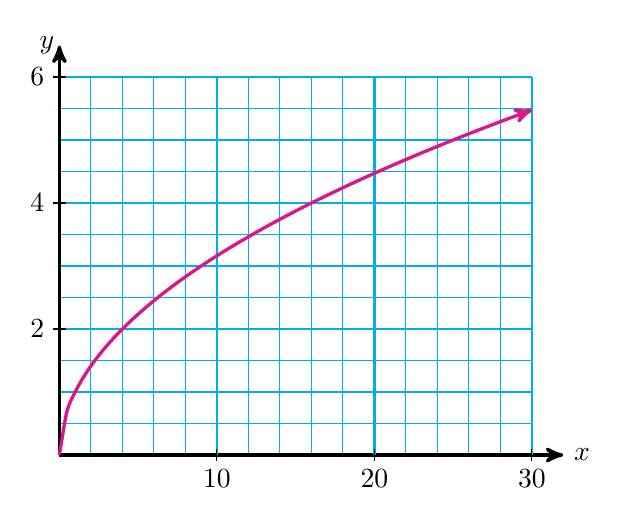
\begin{tikzpicture}[scale=.4]
\draw[cyan] (0,0) grid (15,12);
\draw[black, very thick, ->, >=stealth'] (0,0)--(16,0) node[right]{$x$};
\draw[black, very thick, ->, >=stealth'] (0,0)--(0,13) node[left, xshift=2]{$y$};
\foreach \x [evaluate=\x as \xi using int(2*\x)] in  {5,10,15} {
 \draw[cyan,  thick] ({\x},0) --++(0,12);
 \draw[black] ({\x},.2) --++(0,-.4) node[below, yshift=-2, fill=white, inner sep=1]   {$\xi$};
}
\foreach \x [evaluate=\x as \xi using int(\x /2)] in  {4,8,12} {
 \draw[cyan,  thick] (0,\x) --++(15,0);
 \draw[black] ({.2},\x) --++(-.4,0) node[left, xshift=-2, fill=white, inner sep=1]   {$\xi$};
}
\draw[samples=65,domain=0:15,smooth,variable=\x,magenta!90!black, very thick,->, >=stealth'] plot ({\x},{ sqrt(8)*sqrt(\x)});
\end{tikzpicture}
\newline



hp-9-5-7 semicircle

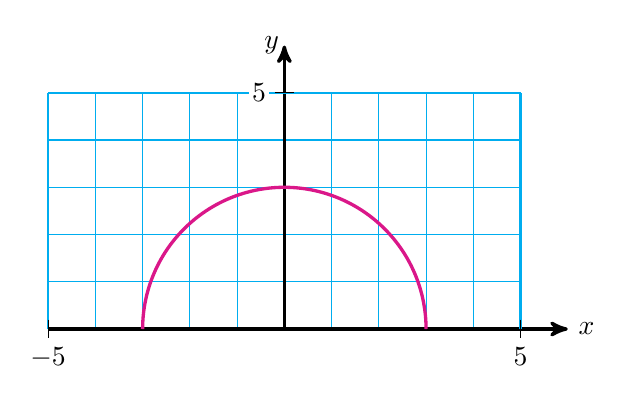
\begin{tikzpicture}[scale=.6]
\draw[cyan] (-5,0) grid (5,5);
\draw[black, very thick, ->, >=stealth'] (-5,0)--(6,0) node[right]{$x$};
\draw[black, very thick, ->, >=stealth'] (0,0)--(0,6) node[left, xshift=2]{$y$};
\foreach \x  in  {-5,5} {
 \draw[cyan,  thick] ({\x},0) --++(0,5);
 \draw[black] ({\x},.2) --++(0,-.4) node[below, yshift=-2, fill=white, inner sep=1]   {$\x$};
}
\foreach \x  in  {5} {
 \draw[cyan,  thick] (-5,\x) --++(10,0);
 \draw[black] ({.2},\x) --++(-.4,0) node[left, xshift=-2, fill=white, inner sep=1]   {$\x$};
}
\draw[samples=65,domain=0:180,smooth,variable=\x,magenta!90!black, very thick] plot ({3*cos(\x)},{3*sin(\x)});
\end{tikzpicture}
\newline


hp-9-5-21 grid

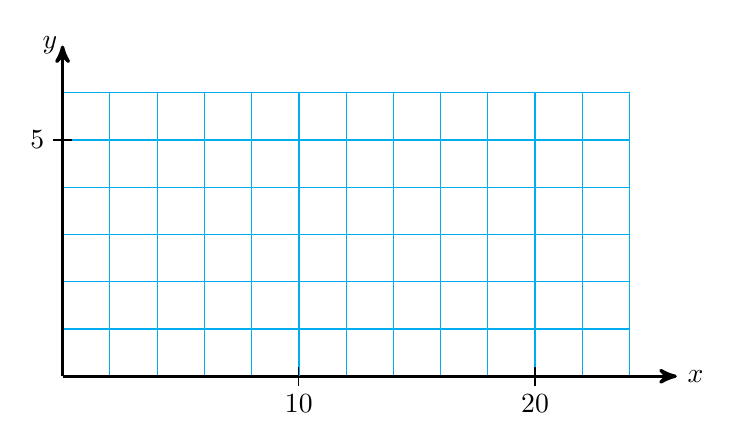
\begin{tikzpicture}[scale=.6]
\draw[cyan] (0,0) grid (12,6);
\draw[black, very thick, ->, >=stealth'] (0,0)--(13,0) node[right]{$x$};
\draw[black, very thick, ->, >=stealth'] (0,0)--(0,7) node[left, xshift=2]{$y$};
\foreach \x [evaluate=\x as \xi using int(2*\x)] in  {5,10} {
 \draw[cyan,  thick] ({\x},0) --++(0,6);
 \draw[black] ({\x},.2) --++(0,-.4) node[below, yshift=-2, fill=white, inner sep=1]   {$\xi$};
}
\foreach \x  in  {5} {
 \draw[cyan,  thick] (0,\x) --++(12,0);
 \draw[black] ({.2},\x) --++(-.4,0) node[left, xshift=-2, fill=white, inner sep=1]   {$\x$};
}
\end{tikzpicture}
\newline



hp-9-5-21ans square root

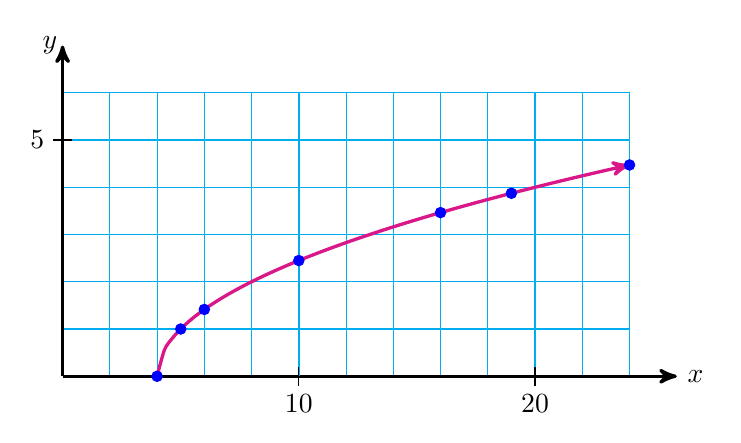
\begin{tikzpicture}[scale=.6]
\draw[cyan] (0,0) grid (12,6);
\draw[black, very thick, ->, >=stealth'] (0,0)--(13,0) node[right]{$x$};
\draw[black, very thick, ->, >=stealth'] (0,0)--(0,7) node[left, xshift=2]{$y$};
\foreach \x [evaluate=\x as \xi using int(2*\x)] in  {5,10} {
 \draw[cyan,  thick] ({\x},0) --++(0,6);
 \draw[black] ({\x},.2) --++(0,-.4) node[below, yshift=-2, fill=white, inner sep=1]   {$\xi$};
}
\foreach \x  in  {5} {
 \draw[cyan,  thick] (0,\x) --++(12,0);
 \draw[black] ({.2},\x) --++(-.4,0) node[left, xshift=-2, fill=white, inner sep=1]   {$\x$};
}
\draw[samples=65,domain=2:12,smooth,variable=\x,magenta!90!black, very thick,->, >=stealth'] plot ({\x},{ sqrt(2*\x-4)});
\foreach \x in {4,5,6,10,16,19,24} {
 \filldraw[blue] ({\x/2}, {sqrt(\x-4)}) circle (1.1mm);
}
\end{tikzpicture}
\newline


hp-9-5-22 grid

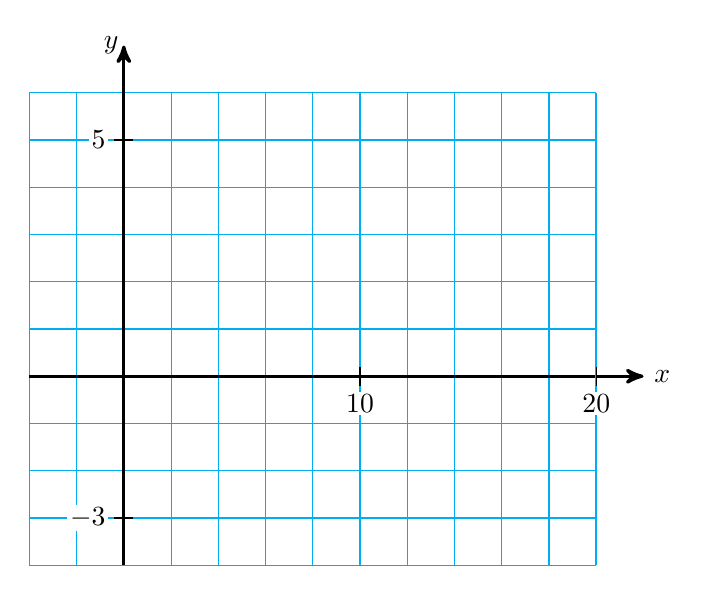
\begin{tikzpicture}[scale=.6]
\draw[cyan] (-2,-4) grid (10,6);
\draw[black, very thick, ->, >=stealth'] (-2,0)--(11,0) node[right]{$x$};
\draw[black, very thick, ->, >=stealth'] (0,-4)--(0,7) node[left, xshift=2]{$y$};
\foreach \x [evaluate=\x as \xi using int(2*\x)] in  {5,10} {
 \draw[cyan,  thick] ({\x},-4) --++(0,10);
 \draw[black] ({\x},.2) --++(0,-.4) node[below, yshift=-2, fill=white, inner sep=1]   {$\xi$};
}
\foreach \x  in  {-3,5} {
 \draw[cyan,  thick] (-2,\x) --++(12,0);
 \draw[black] ({.2},\x) --++(-.4,0) node[left, xshift=-2, fill=white, inner sep=1]   {$\x$};
}
\end{tikzpicture}
\newline






\section{Chapter 9 review}



cr-9-65 right triangle

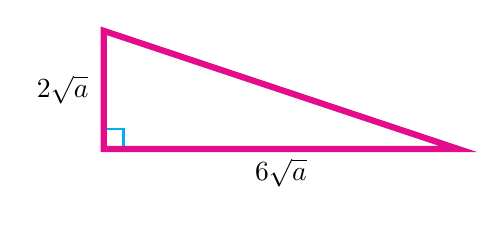
\begin{tikzpicture} 
\coordinate (A) at (0,0);
\coordinate (B) at (4.5,0);
\coordinate (C) at (0,1.5);
\draw[cyan, thick] (A) rectangle ++(.25,.25);
\draw[magenta!95!black,  line width=.8mm] (A)--(B)--(C)--cycle;
\node [left, xshift=-2] at (0,.75) {$2\sqrt{a}$};
\node [below] at (2.25,0) {$6\sqrt{a}$};
\end{tikzpicture}
\newline


cr-9-66 right triangle

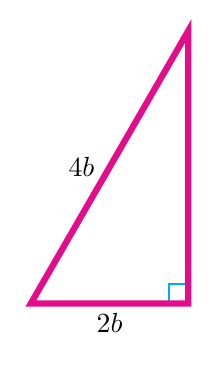
\begin{tikzpicture} 
\coordinate (A) at (0,0);
\coordinate (B) at (2,0);
\coordinate (C) at (60:4);
\draw[cyan, thick] (B) rectangle ++(-.25,.25);
\draw[magenta!95!black,  line width=.8mm] (A)--(B)--(C)--cycle;
\node [left, xshift=-2] at (60:2) {$4b$};
\node [below] at (1,0) {$2b$};
\end{tikzpicture}
\newline



\section{Other stuff}

10 by 10 grid: hp-2-3-12

8 by 8 grid: hp-4-5-17



\end{document}
